\documentclass[
      acmsmall
    , screen
%    , authordraft
%    , anonymous
%    , review=true
  ]{acmart}

% Metadata Information
%\acmConference[DRAFT]{Draft paper}
%\acmJournal{PACMPL}
%\acmVolume{9}
%\acmNumber{4}
%\acmArticle{39}
%\acmYear{2010}
%\acmMonth{3}
%\copyrightyear{2009}
%\acmArticleSeq{9}

% Copyright
%\setcopyright{acmcopyright}
\setcopyright{acmlicensed}
%\setcopyright{rightsretained}
%\setcopyright{usgov}
%\setcopyright{usgovmixed}
%\setcopyright{cagov}
%\setcopyright{cagovmixed}

% DOI
%\acmDOI{0000001.0000001}

% Paper history
%\received{February 2007}
%\received[revised]{March 2009}
%\received[accepted]{June 2009}

\citestyle{acmauthoryear}

%%% PACKAGES %%%

\usepackage[inline]{enumitem}
\usepackage[nomargin,inline,draft]{fixme}
\usepackage{graphicx}
\usepackage{hyperref}
\usepackage{microtype}
\usepackage{pbox}
\usepackage{tikz}
\usepackage{url}
\usepackage{alltt}
%\usepackage[cache=false]{minted}
\usepackage{minted}
\usepackage{syntax}



% Must come after hyperref
\usepackage[capitalise]{cleveref}


%%% FIXME PACKAGE SETUP %%%

\fxusetheme{color}
\fxuseenvlayout{color}

\FXRegisterAuthor{pls}{apls}{\color{teal}[Pablo]}
\FXRegisterAuthor{sjt}{asjt}{\color{magenta}[Simon]}

%%% MINTED COMMANDS FOR HASKELL %%%

\newmint{haskell}{}
\newminted{haskell}{}
\newmintinline{haskell}{}




%%% MACROS %%%

\definecolor{myblue}{rgb}{0.2, 0.3, 1.0}
\newcommand{\bluett}[1]{\textcolor{myblue}{\texttt{#1}}}
\newenvironment{allbluett}{\begin{alltt}\color{myblue}}{\end{alltt}}

\setlength{\itemsep}{2pt}

% Document starts
\begin{document}

% Title portion. Note the short title for running heads
\title
  [Marlowe]
  {Marlowe: financial contracts on blockchain}

\author{Pablo Lamela Seijas}
\affiliation{%
  \institution{University of Kent}
%  \streetaddress{School of Computing}
  \city{Canterbury}
  \state{Kent}
  \postcode{CT2 7NF}
  \country{UK}}
\email{pl292@kent.ac.uk}

\author{Simon Thompson}
\orcid{0000-0002-2350-301X}
\affiliation{%
  \institution{University of Kent}
%  \streetaddress{School of Computing}
  \city{Canterbury}
  \state{Kent}
  \postcode{CT2 7NF}
  \country{UK}}
\email{s.j.thompson@kent.ac.uk}

\begin{abstract}

Blockchains allow the specification of contracts in the form of programs that guarantee their fulfilment. 
Nevertheless, errors in those programs can cause important, and often irretrievable, monetary loss. General-purpose languages provide a platform on which contracts can be built, but by their very generality they have the potential to exhibit behaviours of an unpredictable kind, and are also not easy to read or comprehend for general users. 

An alternative solution is provided by domain-specific languages (DSLs), which are designed to express programs in a particular field. This paper explores the design of one DSL, Marlowe, targeted at the execution of financial 
contracts in the style of Peyton Jones \emph{et al} on blockchains. We have focused on predictability, enforceability, simplicity, 
and ease of analysis and use.

\end{abstract}


% The code below should be generated by the tool at
% http://dl.acm.org/ccs.cfm
% Please copy and paste the code instead of the example below.

%
% End generated code
%

\keywords{
  No keywords
}

\maketitle

% If the default list of authors is too long for headers, it can be redefined
%\renewcommand{\shortauthors}{}

\section{Introduction}



This paper explores the design of a domain specific language, Marlowe,\footnote{Marlowe is named after Christopher Marlowe, the Elizabethan poet, dramatist and spy, who was born and educated in Canterbury, which is also where our university is based. \url{https://en.wikipedia.org/wiki/Christopher_Marlowe}}\footnote{The code for Marlowe is available from \url{https://github.com/input-output-hk/scdsl}
} targetted at the execution of financial contracts in the style of Peyton Jones, Eber and Seward~\cite{PeytonJones:2000} on blockchains. This work is a part of the Cardano project, and is supported by IOHK.\footnote{\url{https://iohk.io}}

In doing this we are required to refine the model of contracts in a number of ways in order to fit with a radically different context. Let us the following example of an ``escrow'' contract we can explain the motivation more concretely. The aim of this contract, written in functional pseudocode in the style of~\cite{PeytonJones:2000} involves three participants \haskellinline{1}, \haskellinline{2} and \haskellinline{3}. Participant \haskellinline{1} is to pay an amount of money to participant \haskellinline{2} on receipt of goods from her. Participant \haskellinline{1} pays the money into escrow controlled by participant \haskellinline{3}. There are two options for the money: if two participants agree to \haskellinline{pay} it to \haskellinline{2}, that goes ahead; if, on the other hand, two of the players opt to \haskellinline{refund} the money to \haskellinline{1}, that is done instead. The \haskellinline{When} construct ensures fires when its first argument -- a condition -- becomes true; the second argument, a \haskellinline{Contract} itself, is then performed, and this makes the payment according to the players' \haskellinline{Choice}.

\begin{haskellcode}
(When (Or (two_chose 1 2 3 refund)
          (two_chose 1 2 3 pay))
      (Choice (two_chose 1 2 3 pay)
              (Pay 1 2 AvailableMoney)
              redeem_original))
\end{haskellcode}

In the traditional model, enforcement of the contract is the responsibility of the legal system. If participant \haskellinline{1} doesn't pay the money into escrow, or participant \haskellinline{3} chooses to keep it for herself, then we can assume that they can be sued for the money and probably damages on top, thus providing both legal and financial incentives for compliance. On the other hand, in the decentralised blockchain model, where there is no central authority, the contract needs to be enforced by design. 

This means that we require participants to commit money to cover all possible expenditure \emph{in advance of the contract executing}. In order to make sure that player continue to engage with a contract we ensure urgency by imposing timeouts: money is committed for a finite period, for example, and when waiting for a player to make a commitment we also impose a timeout to ensure that the contract does not become stuck even if one or more of the participants stops interacting with it.

Moreover, there is not a single blockchain model, and we give a brief overview of the different mechanisms for scripting on blockchain (although this is not the primary purpose of this article). 
A particularly important technical distinction here is that between an account-style model as used by Ethereum~\cite{EthereumRationale}, and the unspent transaction output (UTxO) model of bitcoin~\cite{sok}. 
There is also the question of how precisely the execution of the contract interacts with the blockchain, and how information is to be recorded on the chain. Finally, should the execution ``push'' for changes  to happen, or do external actors have to ``pull'' to effect changes enabled by execution of the contract?

The paper describes version 1.2 of Marlowe, and it should be seen as a work in progress. We have designed it to provide financial contracts in Cardano, but also in order to start to answer the twin
 questions of what smart contracts will look like in Cardano, and how those contracts will be implemented in the overall system.

The paper is structured like this: we begin in Section \ref{section:design} with a discussion of the design rationale for Marlowe, including an overview of the various approaches to scripting in blockchain as well as the different designs of the blockchains themselves. We conclude Section \ref{section:design} with a set of decisions about the blockchain environment for Marlowe. The central part of the paper is Section \ref{section:model} where we introduce the Marlowe model, including the assumptions made in designing 
it, the types of the principal functions and a description of the DSL as an algebraic type, constructor by constructor. 
Section \ref{section:example-saving} presents an example of a larger Marlowe contract, for incentivised saving. Section \ref{section:example-escrow} revisits the escrow example, and shows how it is described using a combination of Marlowe and Haskell constructs: that is, we use Marlowe as an embedded DSL. Section 
\ref{section:tool} introduces Meadow, our tool for visualising and interacting with Marlowe contracts.
Section \ref{section:reflection} reflects on the system design, and observes some alternative designs and Section \ref{section:next-steps} enumerates the next steps for the project.



\section{Design rationale}
\label{section:design}

\medskip
\noindent
In this section we look at existing work on smart contracts and blockchains in general, before exploring the rationale for building the Marlowe language.

\subsection{Smart contracts on blockchains}

As more than one wag has observed, many of the programs that run on blockchains are neither smart nor indeed form 
contracts in any real sense. Nonetheless, this terminology has stuck, and has become shorthand for ``programmed 
interactions on the blockchain''. In an earlier paper, we presented a survey of the approaches 
available~\cite{cryptoeprint:2016:1156}; we give an overview here.

Blockchains are executed in a replicated form by parties who cannot be guaranteed not to be hostile, either by directly trying to change the contents of the chain, or through trying to affect other properties of the chain by indirect means (such as swamping honest parties with work). Programming on the blockchain therefore needs to be constrained in some ways, since it has to be amenable to replication or verification within a reasonable time if the security and integrity of the chain are to be preserved. We look at representatives of the main approaches now.

\paragraph{Bitcoin script}

One approach to this is to choose mechanisms such as bitcoin script~\cite{BitcoinWikiScript} which are manifestly 
non-Turing complete. A bitcoin script, written in a Forth-like language, is essentially linear: it can branch, but the 
language contains neither looping constructs nor recursion. It is therefore straightforward not only to see that scripts 
will terminate, but also to give an accurate estimate of the time taken to execute a script. 

\paragraph{Ethereum}

On the other hand, the Ethereum system~\cite{wood2014ethereum} provides a Turing-complete language for the EVM virtual 
machine, and a higher-level programming language, Solidity, that compiles into EVM code. However, EVM and Solidity 
programs are constrained \emph{post hoc} by two mechanisms: program execution must be paid for using `gas' proportional 
to the effort expended, and a set of \emph{ad hoc} limits on program execution, e.g.\ on stack size.

\paragraph{Nxt}

In Nxt~\cite{Nxt}, programmability of the system is provided through a ``fat'' high-level 
API, which is accessible from Nxt clients through a REST interface. The API provides functionality supporting various 
kinds of transactions. The core software itself doesn't support any form of scripting language; rather, users are 
expected to work with the built in transaction types and transactions that support some 250 primitive operations; these 
can be ``scripted'' in a client (only) using a binding to the API, which is available, for instance, in JavaScript.

\paragraph{Multiple languages}

A common feature of many blockchain platforms is that they provide multiple scripting languages. As we noted earlier, Ethereum can be programmed at the EVM level as well as by using the high-level Solidity language. Tezos~\cite{tezos-white-paper} supports the stack-based, strongly-typed, functional language Michelson, but also provides a high-level language, Liquidity, that compiles into Michelson. Liquidity is also functional and strongly typed, but provides more constructs in a more familiar syntax, namely that of a subset of OCaml. 

The \ae{}ternity system~\cite{aeternity} provides multiple languages and VMs:\footnote{As presented by Erik Stenman at CODE BEAM SF, March 2018, \url{https://www.youtube.com/watch?v=VXsqvfPIdWg}} the functional language  Sophia (akin to Reason) and the Functional Typed Warded Virtual Machine (FTWVM) for safe ``system level programming'', the language Varna and the HLM for simple contracts, and a (port of) Solidity and the EVM for compatibility with Ethereum. In a similar way, Cardano provides support for IELE~\cite{IELE}, a rational reconstruction of the EVM, and thus for Solidity contracts too. 

\paragraph{Domain-specific languages} 

A domain-specific language or DSL is a high-level language designed to work in a specific field or domain. The intention 
is that because the users will know about the field, the constructs of the language can be designed to be meaningful to 
them, and also that, because of its nature, the DSL need not include all the features of a general purpose language. 
Removing this clutter and having the remaining operations directly reflect the application area is intended to make the 
language more accessible to domain experts who do not necessarily see themselves as programmers.

Stand-alone DSLs have the advantage of providing appropriate, domain-level error messages when things go wrong, but suffer the disadvantage of having to be implemented from scratch. An alternative to this are \emph{embedded} DSLs (EDSLs), which provide a ``little language'' for the particular domain embedded within a general-purpose host language. This means that parts of the host -- such as arithmetical expressions, or list idioms --  can be used to extend the expressibility of the DSL. A notable example of this is the financial contracts language described by Peyton Jones and his collaborators~\cite{PeytonJones:2000}, which is embedded in Haskell.

\paragraph{Other approaches}

There are a variety of other approaches to scripting, including business process notations, such as the OMG's BPMN; 
process calculi such as Rholang; logic rules (in Formal Contract Logic), and finite state machines. More details of 
these are provided in~\cite{cryptoeprint:2016:1156}.

\paragraph{Related work}

The Findel project~\cite{findel} examines financial contracts on the Ethereum platform, based on the seminal~\cite{PeytonJones:2000}, and the authors note that payments need to be bounded; this is made concrete in our account by our notion of commitments. They take no account of commitments or timeouts as we do below, but it should be noted that the Ethereum platform is more powerful than the one that we target in this paper.


\subsection{Blockchain platforms: Cardano and others}

There is not a single model of how a blockchain operates, and in this section we look at some of the tradeoffs possible in this space. This allows us to give a context to some of the design decisions taken in designing Marlowe.  

\paragraph{UTxO and accounts}

The simplest blockchain is Bitcoin. Transactions on Bitcoin are made by spending the (as yet) unspent outputs of 
previous transactions (`unspent transaction outputs' or UTxOs). The chain need not maintain any state, such as the 
current value owned by any particular participant: such \emph{account} information is implicit and external to the 
Bitcoin blockchain. On the other hand, the Ethereum model explicitly keeps track of account values, and so this 
information needs to be kept as state information on chain. While it is possible to translate between UTxO-based and 
account-based chains \sjtnote{cite Bruno paper} the UTxO model is more fundamental, and requires less support from the 
implementation of the chain itself.

\paragraph{Interaction modality}

Contracts can be conceived of as acting in two ways. In a \emph{push} model, contracts are seen to be pro-active, and to 
make things happen. In the case of blockchain, this would include making payments or transactions happen. 
Alternatively, in the \emph{pull} model, contracts enable certain things to happen, such as transactions, but the 
transactions need to be effected by an external player. The pull model makes fewer demands on the blockchain 
implementation than the push model, which requires the contract to be triggered automatically.

\paragraph{Layered design and sidechains}

Some chains have a layered design, in particular Cardano~\cite{cardano}. The Cardano Settlement Layer (SL) is to support settlement of transactions but nothing more complicated, whereas the Computation Layer (or CL) supports more powerful general computations over the chain. Moreover, the Cardano roadmap~\cite{cardano-rationale} envisages the possibility of computation taking place, in part at least, on a sidechain rather than on the main chain itself, which may support only the SL. Other off-chain approaches include the Lightning network, overlaid on blockchains (usually Bitcoin) and the channels of \ae{}ternity, introduced below.

\subsection{Designing Marlowe}

In designing, Marlowe we have chosen a number of options; this description applies to Marlowe version 1.2 

\paragraph{Pull} 

While earlier versions used a ``push'' model of operations, we have revised the language to give a ``pull'' semantics. 
This means, for example, that the language can \emph{enable} a payment to be made, but cannot make the payment happen. 
It is up to the interested party (or parties) to make the change happen. It is therefore possible for the payment not to 
happen, despite the fact that this is against the interest of the receiving party.


\paragraph{UTxO vs.\ accounts}

The language semantics is described in terms of \emph{commitments} of sums of cryptocurrency -- which we choose to 
abbreviate to ``cash'' or ``money'' -- and so is agnostic of the underlying implementation.  However, the current 
redemption mechanism in Plutus Core is not strong enough to support Marlowe, and we are actively investigating the best 
way to extend this mechanism to implement Marlowe in full on Plutus Core.

\paragraph{DSL or EDSL?}

Marlowe is described as an algebraic \haskellinline{data} type in Haskell, and as such can be seen as a simple EDSL. Note, however, that the implementation presented here is for the purposes of presenting the semantics and behaviour of the language in the abstract. The implementation on the Cardano platform could be stand-alone, but more likely it will be a DSL embedded in Plutus or Plutus Core. The details of this remain to be decided, as noted in the introduction.

\begin{figure}[t]
\begin{center}
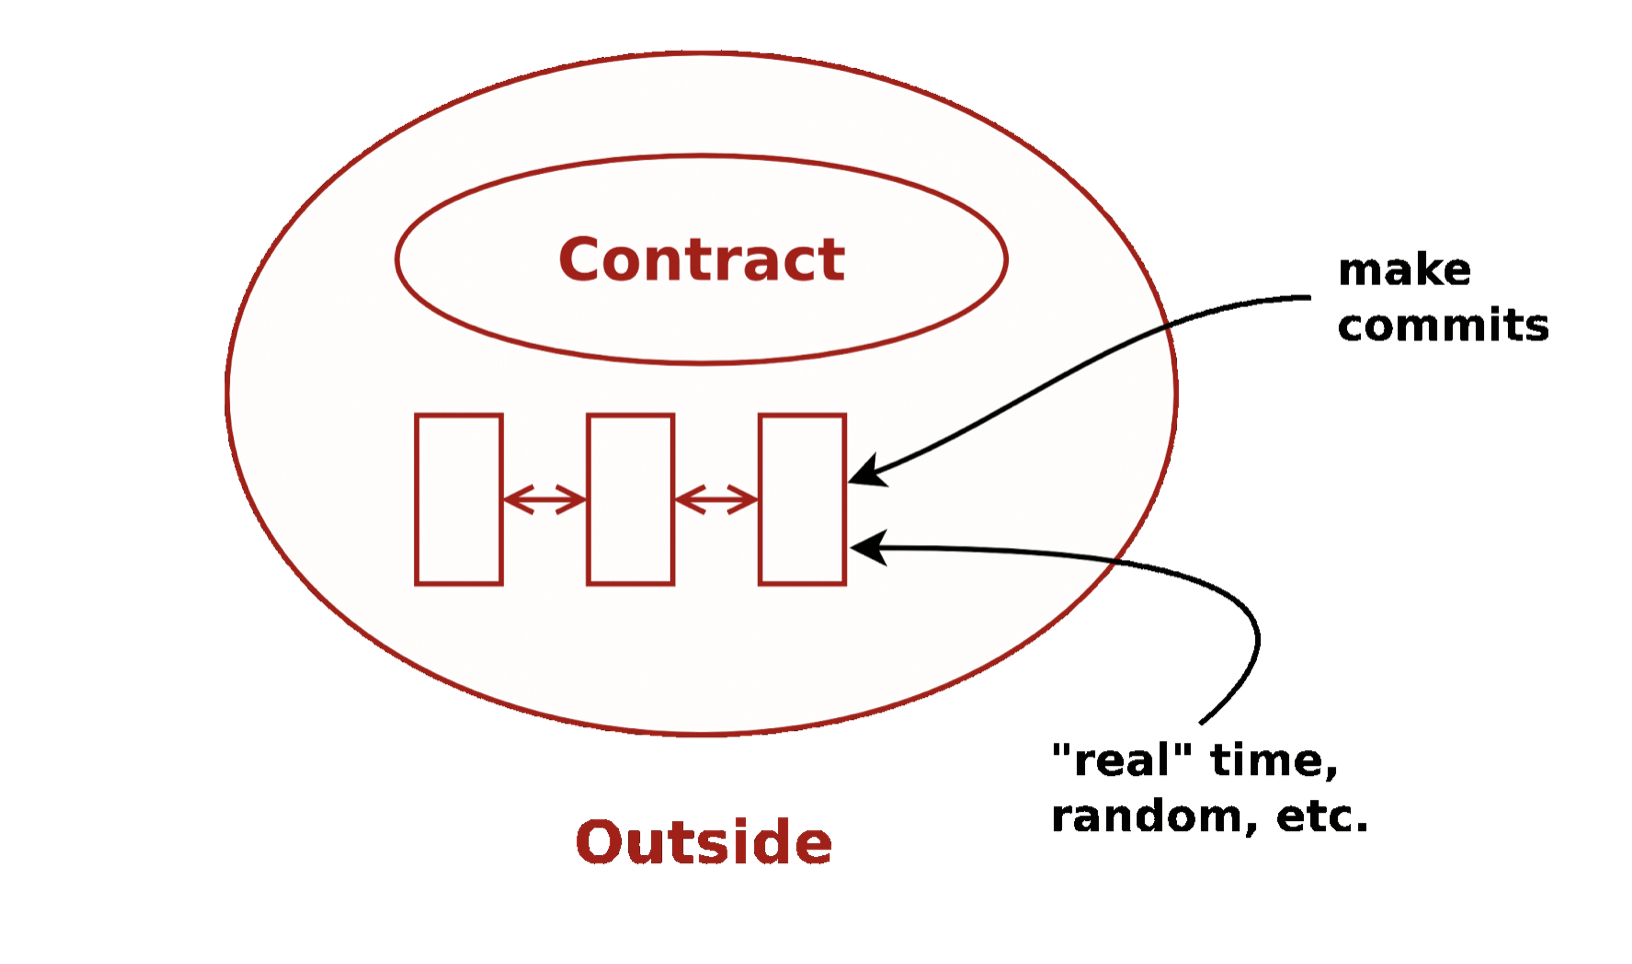
\includegraphics[width=0.6\textwidth]{pix/context.png}
\caption{The context for the contract}
\label{fig:context}
\end{center}
\end{figure}


\section{The model}
\label{section:model}

The DSL is modelled as an algebraic type in Haskell, together with an executable small-step semantics. 
We start by looking at the different types used by the model, then we look at the \haskellinline{Contract} DSL itself, and finally we give its semantics in Haskell. Section \ref{section:example-saving} gives an example of Marlowe in action, and Section
\ref{section:example-escrow} shows the advantage of seeing Marlowe as a DSL embedded in Haskell.

\subsection{The model types}

A running contract will interact with its environment in two ways, as shown in Figure \ref{fig:context}.

\paragraph{Observables}


First, it will need to observe different kinds of varying quantities including, for example, the current time, the current block number and, random numbers, as well as ``real world'' quantities like ``the price of oil'' or ``the exchange rate between currencies A and B''. Each instance of such an observable will be recorded on the blockchain to allow the computation to be repeated for verification purposes. It is assumed that at each step of the execution of the contract, the values of some observables will be needed, and these values are (together) given by a value of type \haskellinline{OS}. Note that these values are not determined by the participants in the contract, but rather by the external environment.

As the examples illustrate, observables come both from aspects of the blockchain (e.g.\ current block number) and externally. In the latter case it will be necessary to agree a trusted oracle or beacon giving the value, which can then be stored (or a hash stored) on chain.

\paragraph{Inputs}


On the other hand, at each step there are -- potentially, at least -- a variety of inputs available from the participants. These include commitments of currency (or ``cash''), redemption of commitments, and claims of payments by a participant; moreover it is also possible for a participant to input an arbitrary value (which we term a ``choice''). The particular inputs at a given step are described by a value of type \haskellinline{Input}.

\paragraph{Commitments}


While informally we might see a commitment to something as being indefinite, it is important to realise that on blockchain a commitment needs to have a timeout so that progress can be forced in a game. After the timeout period the cash can be refunded through the user creating a transaction to reclaim the cash.
Information about the commitments currently in force forms the \haskellinline{State}, which is (potentially) modified at each execution step. 

Payments can be granted by using committed money, but they must be manually redeemed by the recipient, in the 
same way that cash commitments are redeemed when they expire. The effects of the contract in the blockchain are 
represented by a list \haskellinline{AS} of \haskellinline{Actions} that is derived from the execution of each step of the semantics.

\begin{figure}[t]
\begin{center}
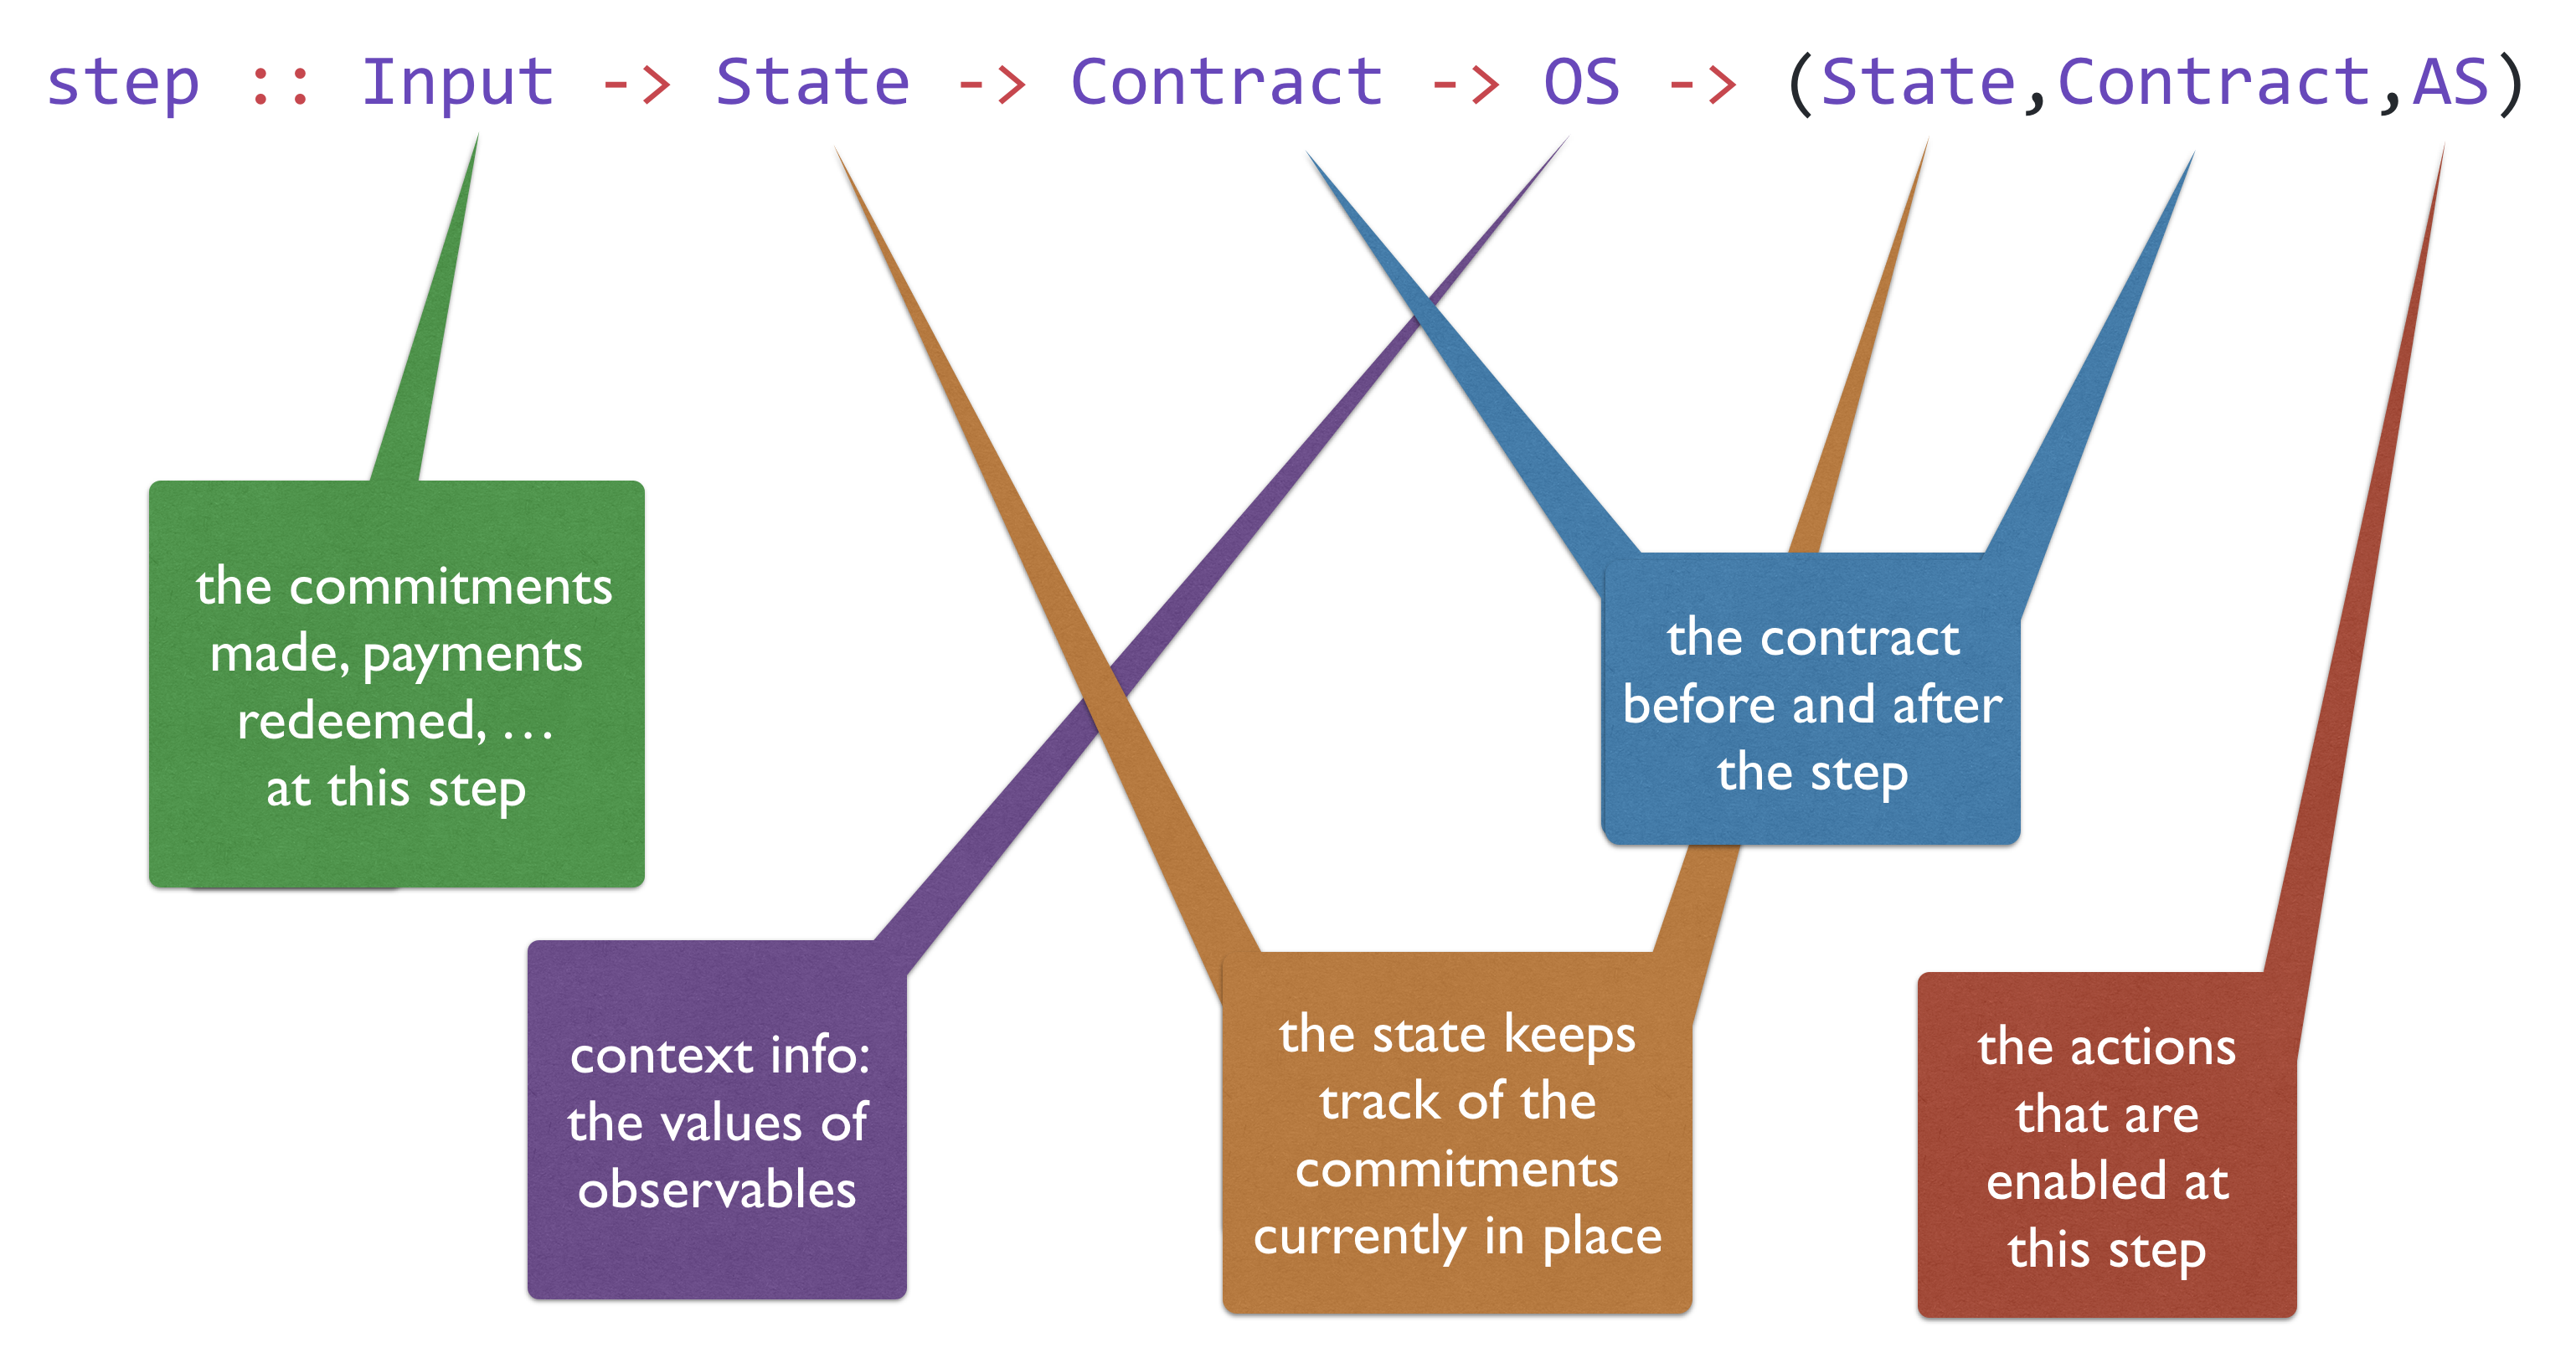
\includegraphics[width=0.8\textwidth]{pix/step-type.png}
\caption{The \haskellinline{step} function}
\label{fig:step-function}
\end{center}
\end{figure}

\paragraph{The \haskellinline{step} function}


This analysis justifies the type of the \haskellinline{step} function:

\begin{haskellcode}
step :: Input -> State -> Contract -> OS -> (State,Contract,AS)
\end{haskellcode}

which is also shown in Figure \ref{fig:step-function}.

\paragraph{Infrastructure}

The model makes a number of assumptions about the blockchain infrastructure in which it is run.

\begin{itemize}
\item It is assumed that cryptographic functions and operations are provided by a layer external to the system, and so they need not be modelled explicitly here.
\item We assume that time is ``coarse grained'' and measured simply by block number, so that timeouts etc.\ are delimited using nothing finer than block number. 
\item Because we assume a ``pull'' model, making a commitment is not something that a contract can perform; rather, it can enable that a commitment is made, but that then has to be established externally: hence the input of (a set of) commitments at each step. The same observation also applies to redeeming a commitment of cash. Commitments that have been made or redeemed need to be recorded somehow.

\item Observables are observed at a particular time and in a particular context. We assume that the recording and 
identification of each (instance of an) observation is provided by the infrastructure of the system. We provide a 
``little language'' for describing observations: \haskellinline{Observation}. 
\item
Similar properties are true for
\haskellinline{Money} amounts: their values are calculated depending on the inputs and state of execution of the 
contract, they can be deterministically established given the context, and they are described through a small 
``expression language''.
\item It is important to be aware that there may be different instances of contracts executed, and for each instance there will typically be different instances of observables (and commitments) observed and recorded.
\item The model manages the release of funds back to the committer when a cash commitment expires (see discussion of the \haskellinline{fullStep} function below).
\end{itemize}

\subsection{The \haskellinline{Contract} type}

The type of contracts is given by

\begin{haskellcode}
data Contract =
   Null |
   CommitCash IdentCC Person Money Timeout Timeout Contract Contract |  
   RedeemCC IdentCC Contract |
   Pay IdentPay Person Person Money Timeout Contract |  
   Both Contract Contract |
   Choice Observation Contract Contract |
   When Observation Timeout Contract Contract   
   \end{haskellcode}
%Originally on "Choice": \footnote{Doesn't the step function need to record what observations are made, so they can be archived in the blockchain? I don't see how your design will support doing so.}\footnote{Yes, we assume that it is part of the infrastructure of this language to record the values of *observables* that are used. However, we have chosen no to make it part of the language itself.}

\subsection{The \haskellinline{step} function}


The \haskellinline{step} function is total, so that for every contract a result of stepping is defined. However, for some kinds of contracts -- commits, redeems or time-shifted contracts -- it is possible that the result of a step is to produce the same contract as the result; such a step is called \emph{quiescent} whereas all other steps \emph{make progress}. We use this distinction in the explanation that follows.


At each computational step, the \haskellinline{step} function is wrapped by a call to the \haskellinline{fullStep} function, which in addition to performing \haskellinline{step} will enable expired cash commitments to be refunded and record any choices made at that step.


The constructors are interpreted like this:

\begin{itemize} 

\item \haskellinline{Null} is the null contract; it will always be quiescent:

\smallskip
\begin{haskellcode}
step _ st Null _ = (st, Null, [])
\end{haskellcode}
\smallskip

\item \haskellinline{CommitCash idCC p v t1 t2 k1 k2}  For this contract to make progress,\begin{itemize}
\item either before the timeout \haskellinline{t1} the user \haskellinline{p} makes a cash commitment of value 
\haskellinline{v} and timeout \haskellinline{t2}  with the identifier \haskellinline{idCC}, 
\item
or the timeout \haskellinline{t1} is exceed:
\end{itemize} 

\smallskip
\begin{haskellcode}
step 
  commits 
  st 
  c@(CommitCash ident person val start_timeout end_timeout con1 con2) 
  os
  | cexe || cexs = (st {sc = ust}, con2, [])
  | Set.member (CC ident person cval end_timeout) (cc commits)
        = (st {sc = ust}, con1, [SuccessfulCommit ident person cval])
  | otherwise = (st, c, [])
  where ccs = sc st
        cexs = expired (blockNumber os) start_timeout
        cexe = expired (blockNumber os) end_timeout
        cns = (person, if cexe || cexs 
                          then ManuallyRedeemed 
                          else NotRedeemed cval end_timeout)
        ust = Map.insert ident cns ccs
        cval = evalMoney st val
\end{haskellcode}
\smallskip
In the first case, a \haskellinline{SuccessfulCommit} action is generated and the contract continues as 
\haskellinline{k1}; in the second case no action is generated and the contract continues as 
\haskellinline{k2}. While neither case holds the contract is quiescent, waiting for the cash to be committed. 

If the cash is committed successfully and the timeout \haskellinline{t2} is reached, then it is impossible to further spend the committed cash, and any unspent funds can be reclaimed by participant \haskellinline{p}.
 This is performed by the \haskellinline{fullStep} function, as noted above.

\item \haskellinline{RedeemCC idCC k} (\haskellinline{CC} stands for cash commitment.) For this contract to make progress, the creator of the cash commitment with identifier \haskellinline{idCC} is required to redeem the unspent funds in that commitment; the contract then continues as \haskellinline{k}, and the action \haskellinline{CommitRedeemed} is produced. 

\smallskip
\begin{haskellcode}
step commits st c@(RedeemCC ident con) _ =
    case Map.lookup ident ccs of
      Just (person, NotRedeemed val _) ->
        let newstate = 
                st {sc = Map.insert ident (person, ManuallyRedeemed) ccs} in
        if Set.member (RC ident person val) (rc commits)
        then (newstate, con, [CommitRedeemed ident person val])
        else (st, c, [])
      Just (person, ManuallyRedeemed) ->
        (st, con, [DuplicateRedeem ident person])
      Nothing -> (st,c,[])
    where
        ccs = sc st
\end{haskellcode}
\smallskip

Committed cash can only be redeemed once, and an attempt to redeem it a second time will produce a  \haskellinline{DuplicateRedeem} action, continuing as \haskellinline{k}.

If the cash commitment with identifier \haskellinline{idCC} has expired, it becomes possible for the remaining funds to be redeemed by the committer; this can be done by the \haskellinline{fullStep} function processing the appropriate \haskellinline{Input}, and an \haskellinline{ExpiredCommitRedeemed} action will be produced. 

Once the commitment \haskellinline{idCC} has expired and is redeemed, a \haskellinline{RedeemCC idCC k} contract will immediately evolve to \haskellinline{k}.
%\footnote{How does the contract determine what actions resulted from a given step? Or is this not required?}
%\footnote{If it is required, restructuring the DSL so that the result action appears as the 'value' of executing a step (using a monadic interface as described for id generation below) would be a good idea.}
%\footnote{We specify the actions generated by each kind of constructor; at each step the list of such actions, of type \haskellinline{AS}, is a component of the result.}. 

\item \haskellinline{Pay p1 p2 v t k} makes it possible, assuming that sufficient funds are available, for 
\haskellinline{p1} to claim  a payment of \haskellinline{v} from \haskellinline{p2} before the timeout 
\haskellinline{t}. The contract continues as \haskellinline{k}. 

\smallskip
\begin{haskellcode}
step inp st c@(Pay idpay from to val expi con) os
  | expired (blockNumber os) expi = (st, con, [ExpiredPay idpay from to cval])
  | right_claim =
    if committed st from bn >= cval
      then (newstate, con, [SuccessfulPay idpay from to cval])
      else (st, con, [FailedPay idpay from to cval])
  | otherwise = (st, c, [])
  where
    cval = evalMoney st val
    newstate = stateUpdate st from to bn cval
    bn = blockNumber os
    right_claim =
      case Map.lookup (idpay, to) (rp inp) of
        Just claimed_val -> claimed_val == cval
        Nothing -> False
\end{haskellcode}
\smallskip

By `available' we mean that sufficient commitments have 
been made and  not yet expired to cover the payment; in this case the payment  uses the currency allocated by the cash 
commitments made by \haskellinline{p1} that expire the earliest.

 This contract will result in a \haskellinline{FailedPay} action if the funds are not available; otherwise a \haskellinline{SuccessfulPay} action is generated.

\item \haskellinline{Both k1 k2} enforces the behaviour of both contracts \haskellinline{k1} and \haskellinline{k2}. 

\smallskip
\begin{haskellcode}
step comms st (Both con1 con2) os =
    (st2, result, ac1 ++ ac2)
    where
        result | res1 == Null = res2
               | res2 == Null = res1
               | otherwise = Both res1 res2
        (st1,res1,ac1) = step comms st con1 os
        (st2,res2,ac2) = step comms st1 con2 os
\end{haskellcode}
\smallskip

Because the model is stateful and produces output actions, to make a step it is necessary to execute a single step of each of  the contracts \haskellinline{k1} and \haskellinline{k2} in sequence: first \haskellinline{k1} then \haskellinline{k2}.

\item \haskellinline{Choice obs k1 k2} behaves as either \haskellinline{k1} or \haskellinline{k2} depending on the (Boolean) result of \haskellinline{obs} at the time that the observation is made, \haskellinline{k1} if it is \haskellinline{True} and \haskellinline{k2} if \haskellinline{False}.

\smallskip
\begin{haskellcode}
step _ st (Choice obs conT conF) os =
    if interpretObs st obs os
        then (st,conT,[])
        else (st,conF,[])
\end{haskellcode}
\smallskip

\item \haskellinline{When obs timeout k def_k} This contract will not progress until \haskellinline{obs} is \haskellinline{True} or until the current block number is greater than or equal to the one specified by timeout. In case the timeout applies, the contract will continue as \haskellinline{def_k}, if the timeout does not apply and \haskellinline{obs} is \haskellinline{True}, then the contract continues as \haskellinline{k}. Otherwise the contract is quiescent.

\smallskip
\begin{haskellcode}
step _ st (When obs expi con con2) os
  | expired (blockNumber os) expi = (st,con2,[])
  | interpretObs st obs os = (st,con,[])
  | otherwise = (st, When obs expi con con2, [])
  \end{haskellcode}
\smallskip

\end{itemize}
We look next at an example of Marlowe in action.


\section{Incentivised saving}
\label{section:example-saving}

In this section, we show how Marlowe can be used for designing a contract that incentivises saving. We use the 
following example: ``participant 2'' offers 20 ADA to ``participant 1'' in exchange for saving 100 ADA for 100 blocks. 
``Participant 1'' will be able to withdraw the savings after block 20, but if that option is chosen, then ``participant 
2'' will not pay the extra 20 ADA to ``participant 1''.

We will start from outer to inner primitives. The first thing is to allow ``participant 1'' to commit the 100 ADA. The 
primitive says that with identity \haskellinline{IdentCC 1} (this is the identity of the commitment), ``participant 
\haskellinline{1}'' can commit \haskellinline{100} ADA before block \haskellinline{10}, and the commitment must 
expire on block \haskellinline{200}. But if the money is not committed before block \haskellinline{10}, then the 
contract will continue as \haskellinline{Null}.

\begin{haskellcode}
CommitCash (IdentCC 1) 1 (ConstMoney 100) 10 200
           step2
           Null
\end{haskellcode}

If the commitment is done correctly and on time, we continue as in \haskellinline{step2}. \haskellinline{step2} is 
another commitment, this time by ``participant 2''. The primitive says that with identity \haskellinline{IdentCC 2},
``participant \haskellinline{2}'' can commit \haskellinline{20} ADA before block \haskellinline{20}, and the commitment
must expire on block \haskellinline{200}. But if the money is not committed before block \haskellinline{20}, then the
contract will continue as \haskellinline{RedeemCC (IdentCC 1) Null}, which in turn gives ``participant 1'' the 
opportunity to withdraw all the money committed immediately.

\begin{haskellcode}
CommitCash (IdentCC 2) 2 (ConstMoney 20) 20 200
           step3
           (RedeemCC (IdentCC 1) Null)
\end{haskellcode}

If the commitment is done correctly and on time, we continue as in \haskellinline{step3}. \haskellinline{step3}
waits until choice with identity \haskellinline{IdentChoice 1} is made by ``participant \haskellinline{1}'' or
until block \haskellinline{100} (whatever happens first). If the choice is made before block \haskellinline{100}, 
it continues as \haskellinline{stepRedeem}, if block \haskellinline{100} comes first, then it continues as 
\haskellinline{step4}.

\begin{haskellcode}
When (PersonChoseSomething (IdentChoice 1) 1) 100
     stepRedeem
     step4
\end{haskellcode}

\haskellinline{step4} pays the \haskellinline{20} ADA committed by ``participant \haskellinline{2}'' in the commit with 
identity \haskellinline{IdentPay 1} to ``participant \haskellinline{1}'', if the payment is claimed before block 
\haskellinline{200}. Once the payment is claimed or after block 200, it continues as \haskellinline{stepRedeem}.

\begin{haskellcode}
Pay (IdentPay 1) 2 1 (ConstMoney 20) 200 stepRedeem
\end{haskellcode}

Finally, \haskellinline{stepRedeem} allows both participants to redeem all the remaining committed funds.

\begin{haskellcode}
Both (RedeemCC (IdentCC 1) Null)
     (RedeemCC (IdentCC 2) Null)
\end{haskellcode}

The whole contract remains as follows:
\begin{haskellcode}
CommitCash (IdentCC 1) 1
           (ConstMoney 100)
           10 200
           (CommitCash (IdentCC 2) 2
                       (ConstMoney 20)
                       20 200
                       (When (PersonChoseSomething (IdentChoice 1) 1)
                             100
                             (Both (RedeemCC (IdentCC 1) Null)
                                   (RedeemCC (IdentCC 2) Null))
                             (Pay (IdentPay 1) 2 1
                                  (ConstMoney 20)
                                  200
                                  (Both (RedeemCC (IdentCC 1) Null)
                                        (RedeemCC (IdentCC 2) Null))))
                       (RedeemCC (IdentCC 1) Null))
           Null
\end{haskellcode}

In the next section, we look at how to take advantage of Haskell embedding when implementing Marlowe contracts.

\section{Marlowe as a DSL embedded in Haskell}
\label{section:example-escrow}

In this section, we give an example of how we can have Marlowe contracts that are easier to write, read, and 
understand, by embedding them into Haskel code (taking advantage that Marlowe contracts are implemented as Haskell 
terms).

The example contract we use through this section implements an escrow contract. Let us imagine that ``participant 1'' 
is buying some item from ``participant 2''. On one hand, if ``participant 1'' pays before receiving the item, there 
is a risk that ``participant 2'' will never give ``participant 1'' the item. On the other hand, if ``participant 2'' 
gives ``participant 1'' the item before ``participant 1'' pays, then there is a risk that ``participant 1'' will never 
pay.

The escrow mechanism allows ``participant 1'' to deposit the money into a contract, in a way that the money will only 
be released when two out of three participants agree on whether ``participant 2'' has indeed given ``participant 1'' 
the item. The third participant (``participant 3'') is supposed to be a neutral third party that will decide in case of 
dispute.

This way, if ``participant 1'' and ``participant 2'' are honest, they will just agree on the result of the transaction 
and ``participant 3'' will not need to do anything. If ``participant 1'' and ``participant 2'' disagree, ``participant 
3'' will be able to choose whether the money must go to ``participant 1'' or to ``participant 2''.

In addition to this, in our implementation, the money paid for the item is 450 ADA, it must be committed by 
``participant 1'' before block 10, and it will be refunded to ``participant 1'' if there is no consensus before block 
90.

We start by defining some Haskell functions. We can encapsulate identifiers in functions to make the contract more 
readable. That way we can generate an identifier for the cash commitment:

\begin{haskellcode}
iCC1 :: IdentCC
iCC1 = IdentCC 1
\end{haskellcode}

And an identifier for the payment:

\begin{haskellcode}
iP1 :: IdentPay
iP1 = IdentPay 1
\end{haskellcode}

We can also create a sub-contract that allows the money to be redeemed by ``participant 1'':

\begin{haskellcode}
redeem_original :: Contract
redeem_original = RedeemCC iCC1 Null
\end{haskellcode}

Each participant has a say on who deserves the money: either ``participant 1'' deserves a refund, which we represent 
with the number $0$; or ``participant 2'' deserves a payment, which we represent with the number $1$. Because there is 
only one choice to make per participant, we use the same \haskellinline{IdentChoice} as their participant id. We can 
define a function that returns an observation that is true if and only if the participant \haskellinline{per} has 
chosen the number \haskellinline{c} as follows:

\begin{haskellcode}
chose :: Int -> ConcreteChoice -> Observation
chose per c = PersonChoseThis (IdentChoice per) per c
\end{haskellcode}

Then we can easily write a function that returns an observation that is true if and only if at least one of the 
participants \haskellinline{per} and \haskellinline{per'} has chosen the number \haskellinline{c} as follows:

\begin{haskellcode}
one_chose :: Person -> Person -> ConcreteChoice -> Observation
one_chose per per' val = (OrObs (chose per val) (chose per' val)) 
\end{haskellcode}

After that, we can write a function that returns an observation that is true if and only if at least 
two of the three participants \haskellinline{p1}, \haskellinline{p2}, and \haskellinline{p3} have chosen the number 
\haskellinline{c} as follows:

\begin{haskellcode}
two_chose :: Person -> Person -> Person -> ConcreteChoice -> Observation
two_chose p1 p2 p3 c = OrObs (AndObs (chose p1 c) (one_chose p2 p3 c))
                             (AndObs (chose p2 c) (chose p3 c))
\end{haskellcode}

Finally, we can write the escrow contract, which would remain as follows:

\begin{haskellcode}
escrow :: Contract
escrow = CommitCash iCC1 1 (ConstMoney 450) 10 100
                    (When (OrObs (two_chose 1 2 3 0)
                                 (two_chose 1 2 3 1))
                          90
                          (Choice (two_chose 1 2 3 1)
                                  (Pay iP1 1 2 (AvailableMoney iCC1) 100
                                       redeem_original)
                                  redeem_original)
                          redeem_original)
                    Null
\end{haskellcode}

The outermost primitive \haskellinline{CommitCash} allows the ``participant 1'' to commit 450 ADA before block 10, 
with the promise that money will be released on block 100 if they are not claimed before that.

The next primitive, \haskellinline{When}, waits for one of three things to happen:
\begin{enumerate}
 \item Two out of three choose $0$.
 \item Two out of three choose $1$.
 \item The block 90 is added to the blockchain.
\end{enumerate}

If the third option happens first, the money is refunded. Otherwise, there is a \haskellinline{Choice} that will 
immediately refund the money to ``participant 1'' unless two out of three chose $1$; in the later case, 
\haskellinline{Pay} will give ``participant 2'' the opportunity to claim the funds available in \haskellinline{iCC1} 
before block 100. If the funds are not claimed before block 100 they will also be refunded to ``participant 1''.

In the next section, we cover the online contract visualisation and interaction tool for Marlowe.

\section{Visualising and interacting with contracts}

\label{section:tool}

One of the objectives of Marlowe is to be accessible to a wider audience
than a general purpose language would. With this aim, and to aid Marlowe's
usage by people that does not know is not familiar with its syntax,
we have developed Meadow, a web tool that supports the interactive construction,
edition, and simulation of smart-contracts written in Marlowe. The
tool is publicly available in the url: \url{https://input-output-hk.github.io/scdsl/}.
In Figure~\ref{fig:full-screenshot-demo}, we provide a screenshot
of Meadow in the middle of simulating the execution of the ``incentivised
saving'' contract described in Section~\ref{section:example-saving}.

Meadow has been mainly written in Haskell and compiled to JavaScript
by the Haste compiler~\cite{Haste}, it also relies on
the Blockly library~\cite{Blockly} for providing a visual
editor for smart contracts written in Marlowe. Blockly's editor allows
the user to visualise and edit smart-contracts as interlocking blocks
that can be dragged and dropped like pieces of a jigsaw puzzle (see
Figure~\ref{fig:detail-of-block}). Meadow also provides functionality
to generate syntactically correct and formatted code (that is displayed
in the upper right corner of the application), and to convert the
code back to its block representation.

\begin{figure}
\begin{centering}
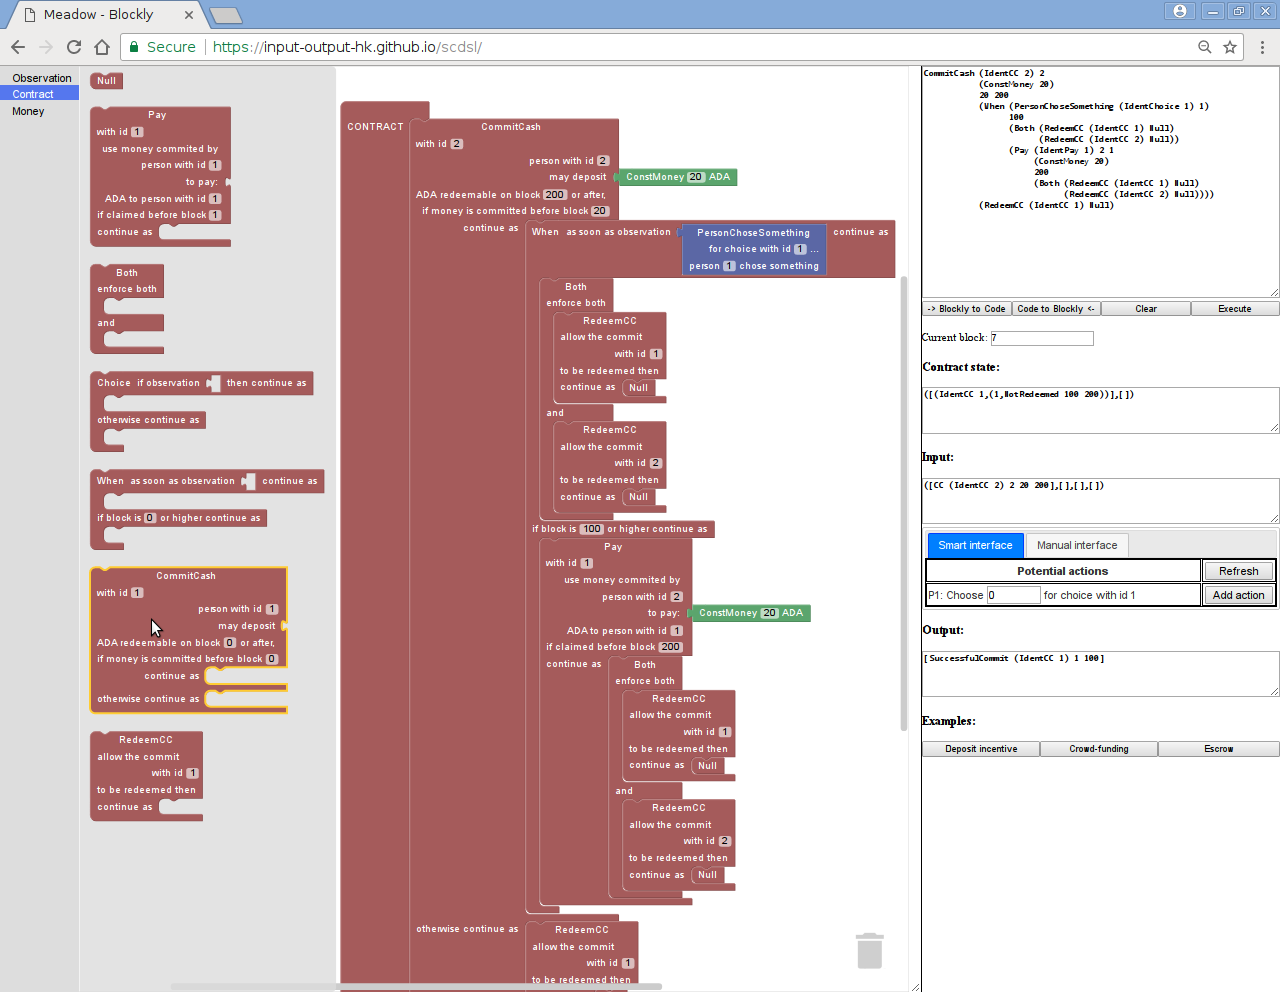
\includegraphics[width=1\textwidth]{pix/screenshot1}
\par\end{centering}
\caption{\label{fig:full-screenshot-demo}Screenshot of Meadow tool
simulating the incentivised deposit contract.}
\end{figure}

\begin{figure}
\centering{}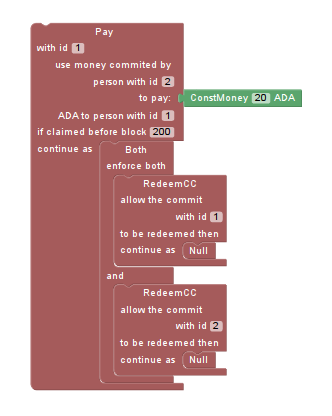
\includegraphics[scale=0.5]{pix/detail1}\caption{\label{fig:detail-of-block}Detail of five interlocked 
blocks.}
\end{figure}

The execution of complete contracts can be simulated block by block
by using the panel on the right (see Figure~\ref{fig:detail-of-interface}),
which includes text fields to view and edit the current block number,
the state of the contract, the current inputs, and the outputs from
last block.

\begin{figure}
\centering{}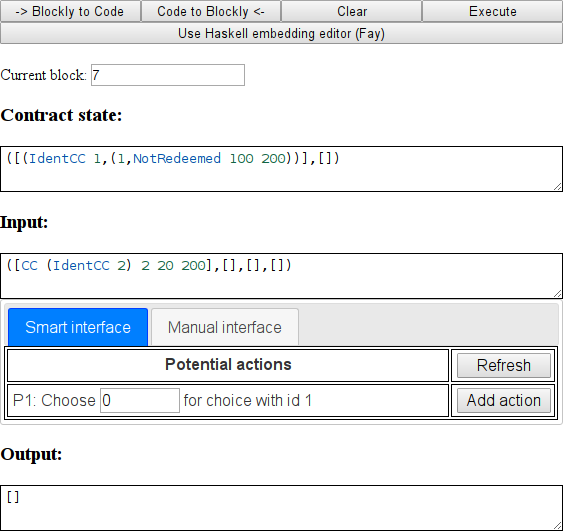
\includegraphics[scale=0.5]{pix/detail2}\caption{\label{fig:detail-of-interface}Detail of the interface for 
contract
execution simulation.}
\end{figure}

Additionally, to facilitate the introduction of inputs, Meadow provides
two different interfaces:
\begin{itemize}
\item The manual interface (see Figure~\ref{fig:detail-of-manual-interface}),
provides a template for each of the four possible types of input:
commits, redeems, payment claims, and choices.
\item The smart interface (see Figure~\ref{fig:detail-of-smart-interface}),
calculates the possible operations that would make sense given the
current inputs, state of the contract, block number, and remaining
contract; and it provides them in a table with most of the parameters
already filled in.
\end{itemize}
\begin{figure}
\begin{centering}
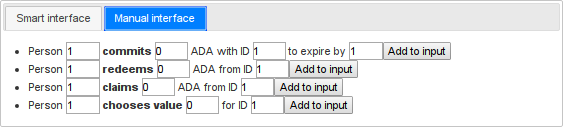
\includegraphics[scale=0.5]{pix/detail3}
\par\end{centering}
\caption{\label{fig:detail-of-manual-interface}Detail of the manual interface.}
\end{figure}

\begin{figure}
\centering{}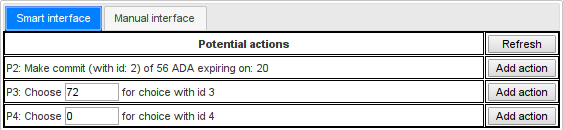
\includegraphics[scale=0.5]{pix/detail4}\caption{\label{fig:detail-of-smart-interface}Detail of the smart 
interface.}
\end{figure}

The smart interface is usually more convenient to use than the manual
interface since the later provides between 3 and 4 fields for each
operation whereas the former ``guesses'' the possible intentions
of the user and usually can input new operations with a single click
(except for choices, which still may require the user to input a number).

In the next section we re-examine the model and the Marlowe language, looking at possible extensions, alternative design decisions and ways in which we can formally analyse Marlowe contracts.

\section{Reflection}
\label{section:reflection}

We have given a concrete model and DSL, namely Marlowe version 
1.2\footnote{\url{https://github.com/input-output-hk/scdsl/releases/tag/v1.2}}.
In this section we examine how the model can be extended, how contacts can be analysed, reflect on different design 
decisions that might be made and discuss some aspects of the implementation of Marlowe within a blockchain environment.

\subsection{Potential additions to the model}

The model that we have discussed so far is deliberately kept as compact as possible. However there are a number of potential extensions to the model which we introduce here. 

\paragraph{Value commitments}

We have examined a single kind of commitment, namely a commitment of a certain amount of currency. In different 
applications, such as on-chain game playing of games like poker, a commitment to a value will be required. A value 
commitment would include a choice of a play in a game, which would be chosen and concealed from the other players until 
a later point in play, when it can be revealed. The paper~\cite{kumaresan2015use} makes use of this and other 
cryptographic primitives to enforce the rules of poker while maintaining the cards of each player secret.

\paragraph{A monadic DSL}

Haskell is a pure functional programming language, and uses the \haskellinline{Monad} type class to encapsulate
operations that can potentially have a side effect. Many introductions to monads exist \cite{wadler1990comprehending} 
but for the sake of this discussion it is enough to think of a value of type \haskellinline{m a} where \haskellinline{m} 
is a monad as a ``computation that results in something of type \haskellinline{a}''. The \haskellinline{Monad} API 
allows such computations to be assembled, and then, once assembled, they may be run, in general causing some 
side-effects as a part of the computation.

We can make the \haskellinline{Contract} type monadic, so that new, unique identifiers are automatically generated. This gives two nice properties. First, they are guaranteed to be unique; secondly they can be generated only in cases where a commit has been made successfully (within the required time period). The 
\haskellinline{do} notation supported by monads allows the generated names to be captured by the \haskellinline{bind} operation and referred to later in the computation.


\subsection{Potential model analyses}
\label{section:analysis}

Given that we have a language and a semantics for it, we can examine its properties. These might be properties of 
individual runs of a particular contract, of all runs of a given contract, or indeed properties of all the contracts of 
the language. In this section, we look at two particularly obvious questions, but these are not the only ones that we 
might ask.



\paragraph{What are the valid contracts?}

One possible definition is ``those contracts that do not lead to a \haskellinline{FailedPay} action''.
Given the mechanisms for making and using commitments are limited by timeouts, it should be possible to write contracts that have this property, perhaps with some assumptions about the value of observables.
Looking at this in a little more detail, we would expect the following points to hold.
\begin{itemize}
\item For a \haskellinline{Pay} contract a sufficient balance not to produce a \haskellinline{FailedPay}.
\item For \haskellinline{Both} we require a sufficient balance for both contracts combined. Need to think here whether the two conjuncts should be independent, or whether a commitment in one half can be used in the other.
\item For \haskellinline{Choice} we require a sufficient balance for the maximum of the requirements of the individual contracts. 
\item For \haskellinline{When}, need to ``age'' the existing commitments relative to the new starting point of the 
continuation contract.
\item \haskellinline{RedeemCC} should not happen twice in any execution, so as to avoid a
\haskellinline{DuplicateRedeem} action.
\item Are there any constraints on \haskellinline{CommitCash} statements? Not directly, but there need to be sufficient 
funds available to pay if needed, and enough time for the commitments to time out.
\end{itemize}

\paragraph{Do all contracts potentially evaluate to \haskellinline{Null}?}

That is, for each contract do there exist sequences of inputs and observables such that stepping the contract with them 
leads to \haskellinline{Null}? Furthermore, do all sequences of inputs and observables eventually evolve to 
\haskellinline{Null}? Some relevant points include:
\begin{itemize}
\item For \haskellinline{When}, in principle, we would need to be able to make \haskellinline{interpretObs st obs os} 
true. However, since there is  a timeout to \haskellinline{When} then there is no need to impose this condition, as we 
will progress at timeout if not before.
\item As we have put timeouts on to \haskellinline{CommitCash} and \haskellinline{Pay}, the only construct that may not 
reduce to \haskellinline{Null} eventually is \haskellinline{RedeemCC}. \haskellinline{RedeemCC} will still reduce to 
\haskellinline{Null} if the commitment that it refers to has expired (and it will produce a 
\haskellinline{DuplicateRedeem} action), but it will be quiescent forever if the money is never comitted in the first 
place.
\item Other constructs will reduce to \haskellinline{Null} eventually as long as their continuations also reduce to 
\haskellinline{Null} (as is the case of \haskellinline{Both}).
\end{itemize}

\subsection{Questions and alternatives}

The model outlined here raises a number of questions, or suggests a number of alternative choices.

\paragraph{Time}

The model does not take time as an observable, but rather it is defined in terms of \haskellinline{BlockNumber} only. We could  use ``slot time'' instead: \emph{``We consider a setting where time is divided into discrete units called slots. A ledger, described in more detail below, associates with each time slot (at most) one ledger block.''}\footnote{\url{https://eprint.iacr.org/2016/889.pdf}}

\paragraph{Timelocks}

In systems where time is significant, it is possible to build ``timelocks'' under which 
it becomes impossible for time to progress. Is it possible for block number to depend on progress of computation? We conjecture not, because otherwise it would be possible to produce timelocks, under which it would become impossible for time to progress. 

\paragraph{Relative time}

Timeouts are expressed in absolute time: presumably they could be relative (with recording on the blockchain of the times at which they are triggered).

\paragraph{Determinism}

The model is deterministic, with all non-determinism being external, and confined to observables. This is surely necessary in order to support computation replay, but does it restrict the expressibility of the model?

\paragraph{Causality}

Is there a notion of causality for these contracts? Would we be able to characterise it semantically? Syntactically?

\paragraph{Expiry}

Does a contract expire if a surrounding commitment does? We have not made this a feature of the model.

\paragraph{Premature repayment}

The \haskellinline{RedeemCC} construct is intended for premature repayment of a cash commitment, i.e. before the commitment has timed out. Alternatively, it would be possible for the underlying model to repay all committed but unspent cash automatically at the end of a contract (but before all commitments have expired), but we might want to do the same thing at the end of each ``round'' of  a game, for instance.

\paragraph{Fungibility}

We have modelled cash as fungible: we make payments using the cash commitments in order of expiry time, with those expiring earliest being used first. Building a model on UTxO might be a reason for using a different approach.


\paragraph{The \haskellinline{Both} construct}

Does the \haskellinline{Both} constructor potentially produce invalid/misleading contracts, combining a commitment in 
one half with its use in the other? The problem is that this might potentially lead to 
a failed payment. 

\paragraph{Monotonicity}

Some observables have a ``monotonicity'' property: once a choice is made, it is fixed forever; on the other hand, something not yet chosen is only so thus far; do we need to reflect this in the observations that we allow?


\subsection{Towards an implementation in Cardano}
\label{section:towards-implementation}

The contracts implemented in the Marlowe language have an implicit interface defined for what would correspond to the 
client side of a distributed application, as shown by the interactive interface. 

\paragraph{Compilation}

We have designed Marlowe assuming that each contract would be compiled into
\begin{itemize} 
\item one or more smart contracts (potentially written in Plutus) and 
\item a client side program or interface that has a limited number of choices to be made at each point in time 
(including an interface for the observables). 
\end{itemize}
Of course, we probably do not want to give a user a programmatic interface but an actual application with user 
interface. So there is still some work to be done to create interfaces on top of the client side of the contracts.

Since the current version of Marlowe follows the `pull' model, a contract written in Marlowe could also be potentially
compiled to a smart-contract written in Ethereum. This could be done in two ways, it could be compiled so that an 
smart-contract represents a single instance of the Marlowe contract (with a fixed set of participants), or 
alternatively it would be possible to create a generic smart-contract with an extra ``instantiate'' operation that 
sets-up a new Marlowe contract instance with a given set of participants (represented by a set of public keys).

\paragraph{Transactions}

In principle, we can directly translate each operation in the model (i.e: cash commitment, payment claim, choice, or
redemption) into a separate transaction in the blockchain. In Ethereum model this would work in the same 
way that is simulated by Meadow: several operations can be issued in parallel and the blockchain subsystem will 
automatically apply them in some order and integrate them into the next block.

Another approach would be to use a UTXO model with continuations in which a UTXO represents a contract. In this model,
an operation would correspond to a transaction that spends a UTXO and creates (at least) a new UTXO that represents the 
contract after the operation.

Usually, in the UTXO model, it is necessary that a UTXO is in the blockchain in order for another transaction to be able 
to spend it. This could potentially limit the number of operations that can be applied in a single block to one, which 
would make infeasible the approach of using the same UTXO to represent several instances of the same contract (since it 
would not scale).

On the other hand, it would prevent non-determinism and, with it, it would remove the possibility of race-conditions. A 
change to the state of a contract before a transaction (and its corresponding operation) is accepted in the blockchain 
would invalidate the transaction and require the user to issue it again.

Even if we only allow one transaction per block, it would still be possible to combine several transactions off-chain 
and to issue a transaction that contains several operations. However, that would require an offline protocol 
independent from the blockchain and it would require participants to collaborate.

\paragraph{Cost}

The Cardano platform has a notion of cost, and Marlowe contracts will potentially incur costs of two kinds:
\begin{itemize} 
\item The cost of a single transaction execution (a single Plutus validator).
\item The cost of the whole contract, which may consist of many transactions.
\end{itemize} 
Even in Ethereum this distinction is important because single contract execution is limited by gas (and is thus finite), whereas the life of the whole contract may be unbounded and consist of an indefinite number of transactions.  So far we are assuming contracts defined in Marlowe to be finite in both aspects. They could be infinite if we were to define them co-inductively as recursive members of the DSL type.

\paragraph{Recording information on chain}

Commitments and values of observables need to be recorded somehow, and this raises the potential issue about bloating 
the chain with data. In general, it will only be necessary to store a signed hash value of the observable, and this will 
keep data usage bounded.


\paragraph{General computations}

If we have contracts that involve, for example, the oil price then we may need to convert a published price in USD into ADA, using a value for the prevailing USD/ADA exchange rate. This will require a computation: in this case, a multiplication. If Marlowe is to be stand-alone then we need to be extend it with arithmetic and other operations, but we expect Marlowe to be embedded in Plutus (Core) and so to be able to use the facilities of the host language here.

\paragraph{Sidechains and wallets}

The implementation may split contract execution between the main chain and a sidechain (or chains). This will allow links from Marlowe to work on securing multiparty sidechain games/contracts (MPCs).


\section{Next steps}
\label{section:next-steps}

We plan to continue the work with Marlowe in a number of directions. First, we need to sign off a definition of the language, as the current status of Marlowe 1.2 is that of a proposal.

\paragraph{Context}

We should decide on the final form of the language -- for example, should it be monadic or not -- and the relation of Marlowe to Plutus (Core). In particular, answering the latter question will require work on the current redeemer/validator model of transactions in Plutus Core.

\paragraph{Implement in Cardano}

An immediate goal is to implement Marlowe in Cardano, noting the observations of Section \ref{section:towards-implementation} and to deploy it in a test network to observe and measure its behaviour in practice.

\paragraph{Compilation}

Marlowe contracts could be generated by a compilation process from `vanilla' financial contracts. This also suggests that models with off-chain enforcement could be investigated too, with an MPC foundation.

\paragraph{Validation and Verification}

Some degree of validation is provided by Meadow presented in Section \ref{section:tool}, albeit for smaller-scale 
contracts, but there is a general question of how properties of contracts can be inferred. One relatively low-cost is to 
use QuickCheck-style property-based testing~\cite{quickCheck}, and properties developed here become candidates for 
fully fledged verification in a formalisation of the (semantics of) Marlowe.

\paragraph{Analysis}

As we noted in Section \ref{section:analysis} we can develop analyses of various aspects of Marlowe contracts. While these might initially be ``pencil and paper'' analyses, we could expect these to be based on a formalisation of the language and its semantics.

\paragraph{Formalisation} 

Marlowe and its semantics could be formalised in a theorem prover such as Isabelle~\cite{IsabelleHOL}, which has been used in the formalisation of language semantics. A formalisation could provide a sanity check on the language definition, as well as formalise proofs of important properties, based on analysis of the contract language.


\section{Acknowledgements}

Thanks to IOHK staff Manuel Chakravarty, Duncan Coutts, Bernardo David, Charles Hoskinson, Aggelos Kiayias, Darryl 
McAdams, Bruno Woltzenlogel Paleo, and Phil Wadler for their collaboration, and to colleagues from the Universities of 
Kent and Leicester for their comments on previous presentations of this work.



\bibliographystyle{ACM-Reference-Format}
\bibliography{paper}

\end{document}
